\documentclass[12pt, letterpaper]{article}

\usepackage{graphicx} % Required for inserting images
\graphicspath{{./images/}}

\usepackage{amsmath, amssymb, amsthm}
\usepackage{circuitikz, subcaption}
\usepackage{textcomp}
\usepackage{gensymb}
\usepackage{titlesec, wrapfig}


\titleformat{\section}
[block]
{\huge\bfseries\center}
{\thesection.\ }
{0pt}
{}

\titleformat{\subsection}
[block]
{\Huge\center}
{}
{0pt}
{}

\titleformat{\subsubsection}
[block]
{\large\bfseries\center}
{}
{0pt}
{}



\title{PHYS4B:\@ Electromagnitism for \\Scientists and Engineers}
\author{Connor Petri}
\date{Winter 2025}

\begin{document}

\maketitle

\pagebreak

\tableofcontents

\pagebreak

\section{Electrostatics}
\subsection{Introduction to Electrostatics}

\hrulefill

\subsubsection*{Charge}

\paragraph*{Definition}
Much like inertia, charge is a fundamental property of matter that describes how an object interacts with 
electric fields. It is measured in Coulombs $[C]$. Practically, charge indicates if the object has an excess 
or deficiency of electrons.

\paragraph*{Quantization of Charge}
Charge is quantized, meaning that it can only exist in discrete values. 
The smallest possible charge is the charge of an electron. Protons and electrons carry equal but opposite charges, 
represented by $e$.

\begin{equation*}
    q = \pm Ne \Longrightarrow e = 1.6 \times 10^{-19}C
\end{equation*}

Where N is any integer. This means that the charge of an object is always a multiple of the charge of an electron.

\paragraph*{Conservation of Charge}
Much like energy and matter, charge is conserved in a closed system. This means that the total charge in a system
will remain constant. 

\begin{equation*}
    \sum q_i = \sum q_f
\end{equation*}


\paragraph*{Conductors and Insulators}
Electrical conductors are materials in which some of the electrons are not bound to atoms and can move relatively freely
through the material. This allows for the easy transfer of charge. Metals are the most common conductors. 
Electrical insulators are materials in which all of the electrons are bound to atoms and cannot move freely. This impededs
the transfer of charge. Glass, rubber, and plastic are common insulators.\\



\subsubsection*{Coloumb's Law}

\paragraph*{Definition}
Coulomb's law describes the fundimental force between 2 charged objects. It is given by the equation:

\begin{equation*}
    F_e = k_e \frac{q_1q_2}{r^2} \Longrightarrow \vec{F}_{12} = k_e \frac{q_1q_2}{r^2}\hat{r}_{12}
\end{equation*}

Where $F_e$ is the electrostatic force in Newtons, $k_e$ is Coulomb's constant, $q_1$ and $q_2$ are the charges of the objects in Coulombs,
$r$ is the distance between the objects in meters, and $\hat{r}_{12}$ is a unit vector pointing from object 1 to object 2.\\

Notice the similarities between Coulomb's law and Newton's law of gravitation. These similarities are because both are fundamental forces of nature.
Both are inverse square laws, meaning that the force between the objects decreases exponentially as the distance between them increases. Both forces are
proportional to a property of matter (mass for gravity and charge for electrostatics) and a constant ($G$ and $k_e$ respectively).\\

The main difference is that electrostatic forces can be attractive or repulsive, while gravity is always attractive. This is because charge can be positive
or negative, while it is (for our purposes) impossible to have negative mass.\\


\subsection{Electric Fields}
\hrulefill

\paragraph*{Definition}
The electric field is a vector field that describes the force experienced by a charge at any point in space. 
It is measured in Newtons per Coulomb $[\frac{N}{C}]$. It is given by the equation:

\begin{equation*}
    \vec{E} = \frac{\vec{F}_e}{q}
\end{equation*}

Where $\vec{E}$ is the electric field in Newtons per Coulomb, $\vec{F}_e$ is the electrostatic force experienced by the
particle in Newtons, and $q$ is the charge of the particle in Coulombs.\\

\subsubsection*{Electric Field Lines}

\paragraph*{Definition}
Electric field lines are a visual representation of the electric field. They are drawn such that the electric field is tangent to the line at any point. 
The electric field lines are drawn such that they point away from positive charges and towards negative charges.

\begin{center}
    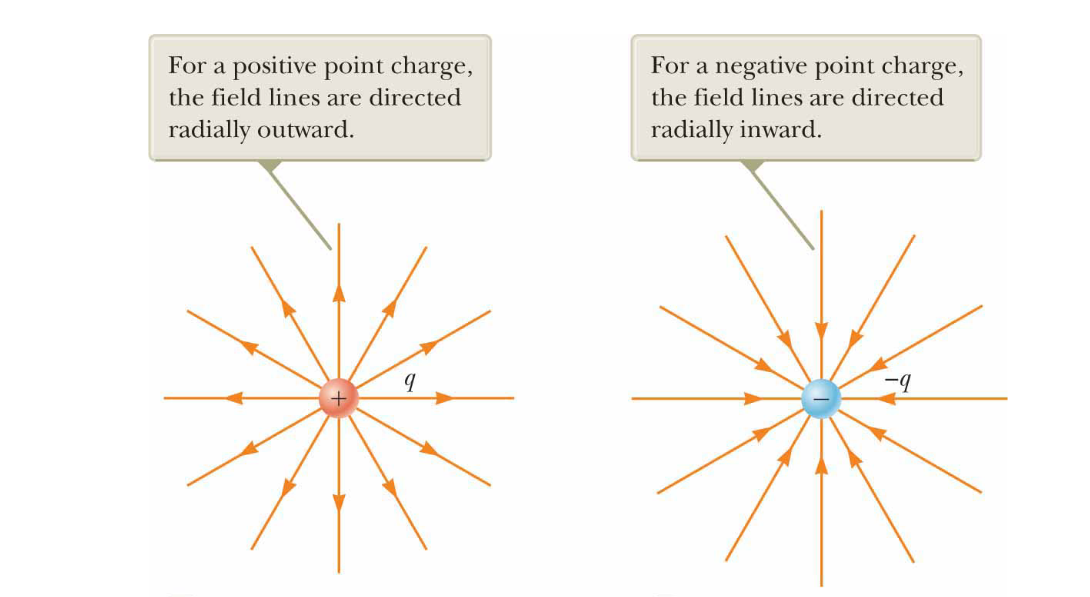
\includegraphics[scale=0.35]{electric_field_lines.png}
\end{center}


The density of the lines leaving or terminating at a particle is proportional to the charge of the particle.

\begin{equation*}
    \frac{N_2}{N_1} = |\frac{q_2}{q_1}|
\end{equation*}

Where $N$ is the number of field lines coming from a charge, and $q$ is the charge of that particle.\\

\begin{figure}[h]
    \centering
    \begin{subfigure}{0.3\textwidth}
        \centering
        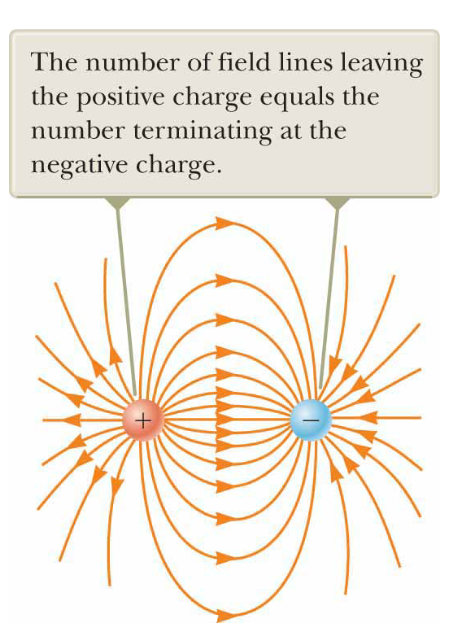
\includegraphics[scale=0.2]{electric_field_lines1.png}
        \caption{Field lines between two equal and opposite charges}
    \end{subfigure}%
    \hspace{0.1\textwidth}
    \begin{subfigure}{0.3\textwidth}
        \centering
        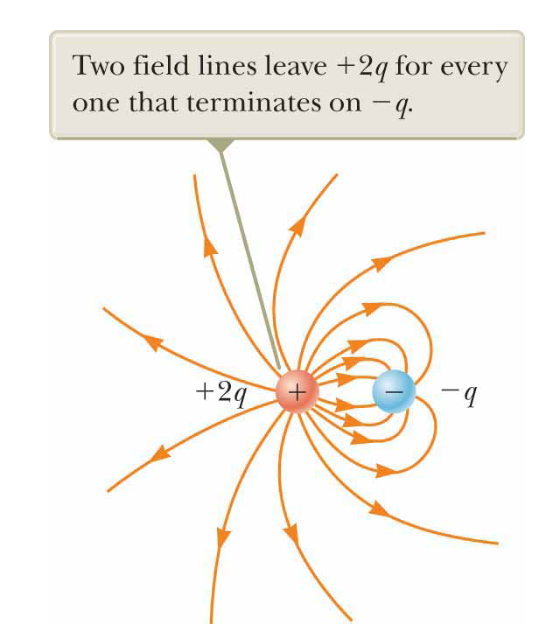
\includegraphics[scale=0.2]{electric_field_lines2.png}
        \caption{Field lines between two unequal and opposite charges}
    \end{subfigure}
\end{figure}

\hrulefill

\subsubsection*{Charge Density}
\paragraph*{Definition}
Charge density is the amount of charge per unit length ($\lambda$), area ($\sigma$), or volume ($\rho$) depending on the geometry of the object.

\begin{align*}
    \text{Linear Charge Density} : \lambda &= \frac{Q}{\ell} \Longrightarrow dq = \lambda d\ell\\
    \text{Surface Charge Density} : \sigma &= \frac{Q}{A} \Longrightarrow dq = \sigma dA\\
    \text{Volume Charge Density} : \rho &= \frac{Q}{V} \Longrightarrow dq = \rho dV
\end{align*}

Where $Q$ is the total charge, $\ell$ is the length, $A$ is the area, and $V$ is the volume of the object.


\subsubsection*{Electric Field Caused by Different Charged Geometry}
\paragraph*{\ \ \ }
Charged objects can have different geometries resulting in different electric fields. Here are some common geometries and their electric fields.

\begin{align*}
    \text{Infinite Line}\ :\ &E_{line} = \frac{\lambda}{2\pi\epsilon_0 r}\\
    \text{Infinite Plane}\ :\ &E_{plane} = \frac{\sigma}{2\epsilon_0}\\
    \text{Parallel Plates}\ :\ &E_{\parallel,plate} = \frac{\sigma}{\epsilon_0}\\
    \text{Ring}\ :\ &E_{ring} = \frac{k_eQx}{(x^2 + a^2)^{3/2}}\\
\end{align*}

Where $\lambda$ is the linear charge density, $\sigma$ is the surface charge density, $k_e$ is Coulomb's constant, $a$ is the radius of the ring, 
$x$ is the distance from the ring, $Q$ is the total charge of the object, and $a$ is the radius of the ring.
\subsection{Electric Flux}
\hrulefill

\begin{figure}[h]
    \centering
    \begin{subfigure}{0.4\textwidth}
        \centering
        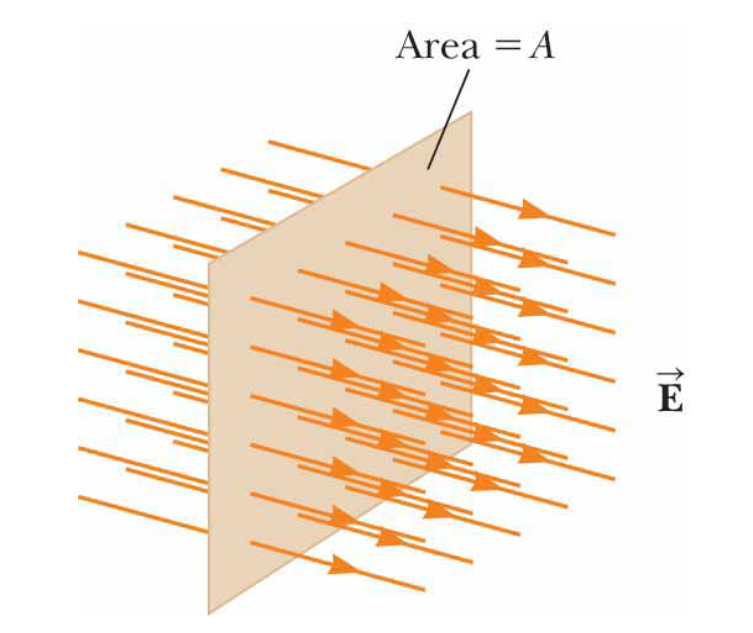
\includegraphics[scale=0.15]{flux.png}
    \end{subfigure}%
    \hspace{0.1\textwidth}
    \begin{subfigure}{0.4\textwidth}
        \centering
        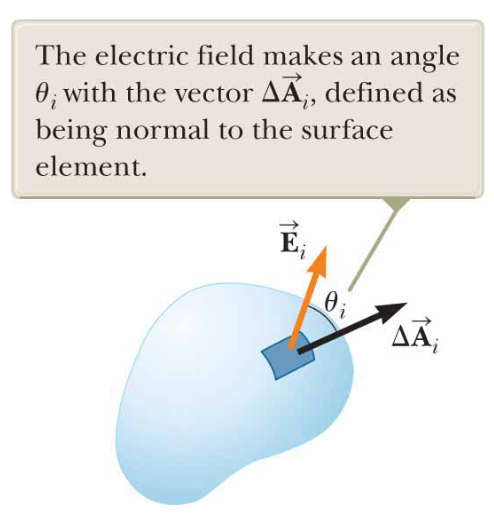
\includegraphics[scale=0.2]{flux1.png}
    \end{subfigure}
\end{figure}

\paragraph*{Definition}
Electric flux is defined as the number of electric field lines passing through a surface. It is measured in Volt meters $[Vm]$.
It is given by the equation:

\begin{equation*}
    \Phi_E = \oint \vec{E} \cdot d\vec{A} = EA\cos(\theta)
\end{equation*}

Where $\Phi_E$ is the electric flux in Newtons per Coulomb, $\vec{E}$ is the electric field in Newtons per Coulomb, $d\vec{A}$ is the differential area vector, and 
$\theta$ is the angle between $\vec{E}$ and $d\vec{A}$.

\hrulefill

\subsubsection*{Gauss's Law}
\paragraph*{Definition}
Gauss's Law states that electric flux through a closed surface is equal to the charge enclosed by the surface divided by the permittivity of free space. This is to say that
any flux generated by electric fields originating from charges outside the surface will cancel out, thus we only care about the enclosed charge.

\begin{equation*}
    \Phi_E = \oint \vec{E} \cdot d\vec{A} = \frac{Q_{\text{enc}}}{\epsilon_0}
\end{equation*}

Where $\Phi_E$ is the electric flux in $Vm$, $\vec{E}$ is the electric field in Newtons per Coulomb, $d\vec{A}$ is the differential area vector, $Q_{\text{enc}}$ 
is the charge enclosed by the surface, and $\epsilon_0$ is the permittivity of free space.
\subsection{Electric Potential}
\hrulefill

\paragraph*{Definition}
Electric potential is the amount of work needed to move a unit charge from a reference point to a specific point in space.
It is measured in volts. The electric potential at a point in space is given by the following equation.

\begin{equation*}
    V = \frac{U_e}{q} = \frac{k_eq}{r}
\end{equation*}

Where $V$ is the electric potential in volts, $U_e$ is the electric potential energy in joules, and $q$ is the charge in coulombs.

\paragraph*{Electric Potential Energy}
Electric potential energy is the energy stored in a system of charges. It is measured in joules. The electric potential energy of a 
system of 2 charges is given by the following equation.

\begin{equation*}
    U_e = q_1V = k_e\frac{q_1q_2}{r}
\end{equation*}

Where $U_e$ is the electric potential energy in joules, $k_e$ is Coulomb's constant, $q_1$ and $q_2$ are the charges in coulombs, and $r$ is the distance between the charges in meters.

\paragraph*{Forces are Derivatives of Potentials}
and the electric force is no different. The electric force is the derivative of the electric potential energy with respect to the distance between the charges. 
We can derive this relationship as follows.

\begin{align*}
    &\quad \vec{F}_e = -\frac{dU_e}{\vec{d\ell}} \quad \Rightarrow \quad \vec{F}_e \cdot \vec{d\ell} = -dU_e \quad \Rightarrow \quad \int \vec{F}_e \vec{d\ell} = -\int dU_e\\
    \Rightarrow& \quad \int \vec{F}_e \vec{d\ell} = -\Delta U_e \quad \Rightarrow \quad W = -\Delta U_e
\end{align*}

Where $\vec{F}_e$ is the electric force in newtons, $\vec{\ell}$ is radial distance from the charge in meters, $\Delta{U_e}$ is the change
in electric potential energy in joules, and $W$ is the work done in joules.

\subsubsection*{Voltage}
Voltage $(\Delta V)$ is the electric potential difference between two points in space. It is measured in volts. The voltage between two points in space is given by the following equation.

\begin{equation*}
    \Delta V = V_b - V_a = \int \vec{E} \cdot \vec{d\ell}
\end{equation*}

Where $\Delta V$ is the voltage in volts, $V_b$ and $V_a$ are the electric potentials at points $b$ and $a$ respectively, $\vec{E}$ is the electric field in newtons per coulomb, 
and $\vec{\ell}$ is the distance between the points in meters.

\paragraph*{Electric Field as a function of Voltage}
The electric field is the derivative of the electric potential with respect to the distance between the charges. We can derive this relationship as follows.

\begin{align*}
    \vec{E} &= \vec{\nabla}V
    \Longrightarrow
    \begin{cases}
        Ex = \frac{\partial V}{\partial x}\\
        Ey = \frac{\partial V}{\partial y}\\
        Ez = \frac{\partial V}{\partial z}
    \end{cases}
\end{align*}

\section{Circuits}
\subsection{Capacitors}
\hrulefill

\paragraph*{Definition}
Capacitors are devices that can store charge. They are made of one or more pairs of conductors seperated by an insulator. 
In circuit diagrams, they are denoted using the following symbol:

\vbox{    
    \center
    \begin{circuitikz}
        \draw (0,0) to[C] (2,0);
    \end{circuitikz}
}

\subsubsection*{Capacitance}

\paragraph*{Definition}
Capacitance is the ability of a capacitor to store charge. It is measured in farads.

\begin{equation*}
    C = \frac{Q}{\Delta V} = \epsilon_0 \frac{A}{d}
\end{equation*}

Where $C$ is capacitance in farads, $Q$ is charge in Coulombs, $\Delta V$ is voltage in volts, $\epsilon_0$ is the 
permittivity of free space, $A$ is the area of the plates in $m^2$, and $d$ is the distance between the plates in meters.


\paragraph*{Electric Field Within a Capacitor}
The electric field within a capacitor is given by the equation:

\begin{equation*}
    E = \frac{\sigma}{\epsilon_0} = \frac{Q}{\epsilon_0 A}
\end{equation*}

Where $E$ is the electric field in $N/C$, $\sigma$ is the charge density in $C/m^2$, $Q$ is the charge in Coulombs, $\epsilon_0$ is the 
permittivity of free space, and $A$ is the area of the plates in $m^2$.\\

Note that any 2 parallel objects with opposite charges can act as a capacitor, for example the sky and the ground during a stormy day.


\paragraph*{Voltage Across a Capacitor}
The voltage across a capacitor is given by the equation:

\begin{equation*}
    \Delta V = Ed = \frac{Qd}{\epsilon_0 A}
\end{equation*}

Where $\Delta V$ is the voltage in volts, $E$ is the electric field in $N/C$, $d$ is the distance between the plates in meters, $Q$ is the charge in Coulombs, $\epsilon_0$ is the permittivity of free space, and $A$ is the area of the plates in $m^2$.\\


\paragraph*{Energy Stored in a Capacitor}
The electric potential energy stored in a capacitor is given by the equation:

\begin{equation*}
    U_e = \frac{1}{2}Q\Delta V = \frac{1}{2}C\Delta V^2 = \frac{Q^2}{2C}
\end{equation*}

Where $U_e$ is the electric potential energy in Joules, $Q$ is the charge in Coulombs, $\Delta V$ is the voltage in volts and $C$ is the capacitance in farads\\

\hrulefill


\subsubsection*{Dielectrics}

\hspace{.5cm} Up until this point, we have made the assumption that the conductors in the capacitor have been seperated by air, however this is not always the case. Dielectrics are insulating materials that are placed between the plates of a capacitor. 
They increase the capacitance of a capacitor by a factor of $\kappa$, or the dielectric constant of that material. $\kappa$ is a direct property of a material that has been determined through experimentation, and thus this value will have to be given
in the problem or retrieved from a table.

\pagebreak

\paragraph*{Capacitance and Electric Field with a Dielectric}
When a dielectric is placed between the plates of a capacitor, the capacitance and electric field change based off of the dielectric constant.

\begin{align*}
    C_\kappa \propto \kappa \\
    E_\kappa \propto \frac{1}{\kappa}
\end{align*}

This changes the equations for capacitance, electric field, and voltage across a capacitor to the following:

\begin{align*}
    C_\kappa = \kappa C_0 = \frac{\kappa Q}{\Delta V}\\
    E_\kappa = \frac{\sigma}{\kappa \epsilon_0} = \frac{Q}{\kappa \epsilon_0 A}\\
    \Delta V_\kappa = E_\kappa d = \frac{Qd}{\kappa \epsilon_0 A}
\end{align*}

\hrulefill


\subsubsection*{Capacitors in Series and Parallel}

\begin{figure}[h]
    \centering
    \begin{subfigure}{.48\textwidth}
        \centering
        \begin{circuitikz}
            \draw (0,2) to[battery] (0, 0)
            (0,2) -- (2,2)
            (2,2) to[C, l=$C_1$] (2,1)
            (2,1) to[C, l=$C_2$] (2,0)
            (0,0) -- (2,0)
            ;
        \end{circuitikz}
        \caption{Wired in series.}
        \label{fig:sub1}
    \end{subfigure}%
    \begin{subfigure}{.48\textwidth}
        \centering
        \begin{circuitikz}
            \draw
            (0,2) to[battery] (0,0)
            (0,2) -- (4, 2)
            (2, 2) to[C, l=$C_1$] (2,0)
            (4,2) to[C, l=$C_2$] (4,0)
            (0,0) -- (4,0)
            ;
        \end{circuitikz}
        \caption{Wired in parallel.}
        \label{fig:sub2}
    \end{subfigure}
    
\end{figure}

\paragraph*{Differences}
Capacitors wired in series and parallel behave differently. Capacitors wired in series carry the same charge, but different voltages.

\begin{equation*}
    q_{eq(s)} = q_1 = q_2 = \cdots = q_n
\end{equation*}

Capacitors wired in parallel behave in the opposite manner, carrying the same voltage, but different charges.

\begin{equation*}
    \Delta V_{eq(\parallel)} = \Delta V_1 = \Delta V_2 = \cdots = \Delta V_n
\end{equation*}
    

\paragraph*{Equivilant Capacitance}
Multiple capacitors can be represented by a single capacitor with an equivilant capacitance. The equivilant capacitance of 
capacitors in series and in parallel is given by the following equations:

\begin{align*}
    \frac{1}{C_{eq(s)}} = \sum_{i=1}^{n} \frac{1}{C_i}\\
    C_{eq(\parallel)} = \sum_{i=1}^{n} C_i
\end{align*}




\subsection{Current and Resistance}

\hrulefill

\subsubsection*{Current}

\paragraph*{Definition}
Current is defined as the time rate of change of charge through an object. It is measured in amps.

\begin{equation*}
    I=\frac{dQ}{dt} \Rightarrow I = nqv_dA
\end{equation*}

Where $I$ is the current in amps $[A] = [\frac{C}{s}]$, $n$ is the free electron density in electrons/$m^3$, 
$v_d$ is the drift velocity in $m/s$, and $A$ is the cross-sectional area of the conductor in $m^2$.


\paragraph*{Drift Velocity}
Electrons are bouncing around randomly. When an electric field is applied, the bouncing is directed 
in a direction, but it is still chaotic. This bouncing results in heat being generated. Heat is defined 
as the kinetic energy of a particle. The speed of the drift of the electrons is called the drift velocity $(v_d)$.

\begin{equation*}
    v_d = \frac{I_{avg}}{nqA} = \frac{I}{nqA}
\end{equation*}

Where $v_d$ is the drift current, $n$ is the free electron density in $\frac{g}{m^2}$, $q$ is the charge of the current carrier 
(usually an electron) in $C$, and A is the cross-sectional area of the conductor in $m^2$.


\paragraph*{Current Density}
Current density is the current per unit area. It can be calculated using the following formula:

\begin{equation*}
    J = \frac{I}{A} = \sigma A = nqv_d
\end{equation*}

Where $J$ is the current density in $Amps/m^2$, $I$ is the current in amps, $A$ is the cross-sectional 
area of the conductor in $m^2$, $\sigma$ is the conductivity of the material, and $n$ is the free electron 
density in electrons/$m^3$.

\pagebreak

Voltage can be calculated as a function of current density and conductivity as follows:

\begin{equation*}
    \Delta V = E\ell = \frac{\ell J}{\sigma}
\end{equation*}

Where $\Delta V$ is the voltage in volts, $E$ is the electric field in volts per meter, $\ell$ is the length of the conductor in meters,


\hrulefill


\subsubsection*{Resistance}

\paragraph*{Definition}
Resistance is defined as the ratio of voltage to current, also known as Ohm's law. It is measured in ohms.

\begin{equation*}
    R = \frac{\Delta V}{I}
\end{equation*}

Where $R$ is the resistance in $\Omega$, $\Delta V$ is the voltage in volts, and $I$ is the current in $A$.


\paragraph*{Resistivity}
Resistivity is the fundimental property of a material that determines how much it resists the flow of current. 
It is measured in ohm-meters $[\Omega m]$.

\begin{equation*}
    \rho = \frac{1}{\sigma} = \frac{RA}{\ell} \Longrightarrow R = \rho \frac{\ell}{A}
\end{equation*}

Where $\rho$ is resistivity in $\Omega m$, $\sigma$ is conductivity in $S/m$, $R$ is resistance in $\Omega$, $A$ is the cross-sectional area of the 
conductor in $m^2$, and $\ell$ is the length of the conductor in meters.\\

\paragraph*{Conductivity}
Conductivity is the inverse of resistivity. It is measured in Siemens per meter $[\frac{S}{m}]$. $[S] = [\frac{1}{\Omega}]$

\begin{equation*}
    \sigma = \frac{1}{\rho} = \frac{\ell}{RA} \Longrightarrow R = \frac{\ell}{\sigma A}
\end{equation*}

Where $\rho$ is resistivity, $\sigma$ is conductivity, R is resistance in $\Omega$, $I$ is current in amps, and $\Delta V$ is voltage in volts.

\paragraph*{Ohmic vs. Non-Ohmic devices}
Ohmic devices are devices that have a Voltage vs Current slope of $\frac{1}{R}$. Non-ohmic devices have a slope that changes with voltage or current.

\paragraph*{Resistivity and Temperature}
The resistivity of a material changes with the temperature of the material. The equation for resistivity as a function of temperature is given by:

\begin{align*}
    \rho_t = \rho_0[1+\alpha\Delta T]\\
    \alpha = \frac{\Delta \rho/\rho_0}{\Delta T}
\end{align*}

Where $\rho_t$ is the resistivity of the material at a given temperature in $\Omega m$, $\rho_0$ is the resistivity of the material at a reference temperature in $\Omega m$, 
$\alpha$ is the temperature coefficient in $\degree C^{-1}$ (a material constant, much like $\kappa$), $\Delta \rho$ is the change in resistivity in $\Omega m$, 
and $\Delta T$ is the change in temperature in $\degree C$.

\hrulefill

\subsection{Electrical Power}


\paragraph*{Definition}
Power is defined as the rate at which energy is transferred or converted. It is measured in watts.

\begin{align*}
    P = \frac{dU_e}{dt} = I^2R = \frac{(\Delta V)^2}{R}
\end{align*}

Where $P$ is power in watts, $U_e$ is electric potential energy in Joules, $\Delta V$ is voltage in volts, and $I$ is current in amps.
\subsection{Direct Current Circuits}
\hrulefill

\subsubsection*{Electromotive Force}
\paragraph*{Definition}
Electromotive force (emf) is the voltage produced by a battery or generator. It is measured in volts. 
The emf of a circuit is the total voltage supplied by the battery or generator.

\begin{align*}
    \Delta V &= \varepsilon - Ir\\
    \varepsilon &= IR + Ir\\
    I &= \frac{\varepsilon}{R+r}
\end{align*}

Where $\Delta V$ is the voltage in volts, $\varepsilon$ is the emf in volts, $I$ is the current in amps, 
and $R$ and $r$ are resistors in ohms.

\begin{figure}[h]
\centering
\begin{circuitikz}
    \draw 
    (0,3.25) to[battery, l=$\varepsilon$] (0,1.75)
    (0,3.25) -- (2,3.25) to[R, l=$R$] (3,3.25) -- (4,3.25)
    -- (4,1.75) -- (3,1.75) to[R, l=$r$] (2,1.75) -- (0,1.75)
    ;
\end{circuitikz}
\end{figure}


\paragraph*{Power}
The power delevered to each of the resistors in the above circuit is given by the following equations.

\begin{align*}
    P_R &= I^2R\\
    P_r &= I^2r
\end{align*}

Note that the specific current value used will depend on how the resistors in the circuit are connected.


\subsubsection*{Equivilant Resistance}

\ \ \ \ Much like capacitors, multiple resistors can be represented by a single resistor with an equivilant resistance. 

\begin{figure}[h]
    \centering
    \begin{subfigure}{0.4\textwidth}
        \begin{circuitikz}
            \draw
            (0,0) node[[font=\footnotesize]label=above:$a$]{} -- (1,0) to[R, l=$R_1$] (2,0) -- (3,0) to[R, l=$R_2$] (4,0) -- (5,0) node[label=above:$b$]{}
            ;
        \end{circuitikz}
    \end{subfigure}
\end{figure}


\paragraph*{In Series}
Resistors in series can be combined into a single resistor with a resistance equal to the sum of the individual resistances.
The current through each resistor in series is the same, but the voltage across each resistor is different.

\begin{align*}
    R_{eq(s)} &= \sum_{i=1}^{n} R_i\\
    I_{eq(s)} &= I_1 = I_2 = \cdots = I_n\\
    \Delta V_{eq(s)} &= \sum_{i=1}^{n} \Delta V_i
\end{align*}

\paragraph*{In Parallel}
Resistors in parallel can be combined into a single resistor with a resistance equal to the reciprocal of the sum of the reciprocals 
of the individual resistances. The voltage across each resistor in parallel is the same, but the current through each resistor is different.

\begin{align*}
    \frac{1}{R_{eq(\parallel)}} &= \sum_{i=1}^{n} \frac{1}{R_i}\\
    I_{eq(\parallel)} &= \sum_{i=1}^{n} I_i\\
    \Delta V_{eq(\parallel)} &= \Delta V_1 = \Delta V_2 = \cdots = \Delta V_n
\end{align*}

\pagebreak


\subsubsection*{Kirchhoff's Laws}

\paragraph*{Junction Rule}
At any junction in a circuit, the sum of the currents must equal zero.

\begin{equation*}
    \sum_{junction} I = 0 \quad \Longrightarrow \quad \sum_{junction} I_{in} = \sum_{junction} I_{out}
\end{equation*}

\paragraph*{Loop Rule}
The sum of the voltages around any closed loop in a circuit must equal zero.

\begin{equation*}
    \sum_{closed loop} \Delta V = 0
\end{equation*}

\paragraph*{Sign Conventions}
\begin{itemize}
    \item If the current enters the positive terminal of a resistor, it is positive.
    \item If the current enters the negative terminal of a resistor, it is negative.
    \item If the current enters the positive terminal of a battery, it is negative.
    \item If the current enters the negative terminal of a battery, it is positive.
\end{itemize}

\hrulefill

\paragraph*{Charging a Capacitor}

\begin{align*}
    Q_{max} &= C\varepsilon\\
    I &= \frac{dq}{dt} = -\frac{q-C\varepsilon}{RC}\\
    q(t) &= C\varepsilon(1-e^{-\frac{t}{RC}}) = Q_{max}(1-e^{-\frac{t}{RC}})\\
    i(t) &= \frac{dq}{dt} = \frac{\varepsilon}{R}e^{-\frac{t}{RC}}\\
\end{align*}


\paragraph*{Discharging a Capacitor}
\begin{align*}
    q(t) &= Q_ie^{-\frac{t}{RC}}\\
    i(t) &= -\frac{Q_i}{RC}e^{-\frac{t}{RC}}\\
\end{align*}


\subsection{RC Circuits}
\hrulefill

\paragraph*{Definition}
An RC circuit is a circuit that contains a resistor and a capacitor. The capacitor stores energy in the form of an electric field, 
while the resistor dissipates energy in the form of heat. The time constant $\tau$ of an RC circuit is given by the product of the 
total resistance and capacitance in the circuit.

\begin{equation*}
    \tau = RC
\end{equation*}

Where $\tau$ is the time constant in seconds, $R$ is the resistance in ohms, and $C$ is the capacitance in farads. 

\paragraph*{Charging a Capacitor}
First, we must update our max charge equation to account for emf.

\begin{equation*}
    Q_{max} = C\varepsilon
\end{equation*}

Where $Q_{max}$ is the max charge the capacitor can hold in Coulombs, C is the capacitance of the capacitor in Farads, and $\varepsilon$
is the electromotive force in volts.\\

We can then find the charge and current of the capacitor as a function of time.

\begin{align*}
    q(t) \quad &= \quad C\varepsilon(1-e^{-t/\tau}) \quad = \quad Q_{max}(1-e^{-t/\tau})\\
    I(t) \quad &= \quad \frac{dq}{dt} \quad = \quad \frac{\varepsilon}{R}e^{-t/\tau} \quad = \quad \frac{q(t) - Q_{max}}{\tau}\\
\end{align*}

Where $q(t)$ is the charge on the capacitor at time $t$ in Coulombs, $I(t)$ is the current through the capacitor at time $t$ in Amps,
$C$ is the capacitance of the capacitor in Farads, $\varepsilon$ is the electromotive force in volts, $R$ is the resistance in ohms,
and $\tau$ is the time constant of the circuit in seconds.

\paragraph*{Discharging a Capacitor}
We can also find the charge and current of a capacitor as it discharges as a function of time.

\begin{align*}
    q(t) &= Q_ie^{-t/\tau}\\
    I(t) &= -\frac{Q_i}{\tau}e^{-t/\tau}\\
\end{align*}

Where $Q_i$ is the initial charge on the capacitor in Coulombs, and the rest of teh variables having the same definition as above.

\section{Magnetism}
\subsection{Magnetic Fields}
\hrulefill

\paragraph*{Definition}
    A magnetic field is a vector field that describes the magnetic influence on moving electric charges, 
electric currents, and magnetic materials. They are generated by moving charges, or current. 
It is represented by the symbol $\vec{B}$ and is measured in teslas (T).\\

    Unlike electric fields, which can be generated by a single source charge, magnetic poles always come in pairs. 
There are no magnetic monopoles. The two types of magnetic poles are called north and south.

\begin{equation*}
    \vec{F}_B = q\vec{v} \times \vec{B}
\end{equation*}

    Where $\vec{F}_B$ is the magnetic force in newtons, $q$ is the charge in coulombs, $\vec{v}$ is the velocity
of the charged in meters per second, and $\vec{B}$ is the magnetic field in teslas.\\

    Note that the magnetic force Insert perpendicular to both the velocity of the charge and the magnetic field. 
This is different from the electric force, which is parallel to the electric field. The direction of the magnetic 
force can be determined using the right hand rule.\\

\begin{center}
    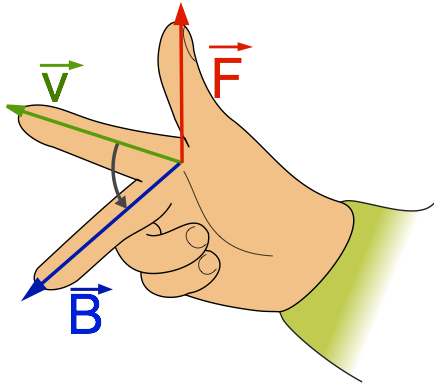
\includegraphics[scale=0.5]{rhr.png}
\end{center}

By convention, $\odot$ represents a vector going into the page, and $\otimes$ represents one coming out of the page.


\paragraph{Charged Particle in a Uniform Magnetic Field}
When a charged particle moves in a uniform magnetic field, it experiences a constant magnetic force that is directed
radially inward. This causes the particle to move in uniform circular motion. We can revise the UCM equations in terms
of the magnetic field and charge of the particle in UCM.

\begin{align*}
    F_B &= qvB = \frac{mv^2}{r}\\
    r &= \frac{mv}{qB}\\
    \omega &= \frac{v}{r} = \frac{qv}{m}\\
    T &= \frac{2\pi r}{v} = \frac{2\pi}{\omega} = \frac{2\pi m}{qB}\\
\end{align*}

Where $F_B$ is the magnetic force in newtons, $q$ is the charge of the particle in coulombs, $v$ is the velocity of the 
particle in meters per second, $B$ is the magnetic field in teslas, $m$ is the mass of the particle in kilograms, $r$ is 
the distance of the particle from the axis of rotation in meters, $\omega$ is the angular velocity in radians per second, 
and $T$ is the period in seconds.\\

\paragraph*{Magnetic Force Acting on a Current-Carrying Wire}
When a current-carrying wire is placed in a magnetic field, it experiences a magnetic force. This force is given by the
following equation.

\begin{align*}
    \vec{F}_B &= I\vec{\ell} \times \vec{B}\\
\end{align*}

Where $\vec{F}_B$ is the magnetic force in newtons, $I$ is the current in amperes, $\vec{\ell}$ is the length of the wire in meters,
and $\vec{B}$ is the magnetic field in teslas. The direction of the force can be determined using the right hand rule.\\

\paragraph*{Torque on a Current Loop in a Magnetic Field}
When a current loop is placed in a magnetic field, it experiences a torque. This torque is given by the following equation.

\begin{align*}
    \vec{\tau}_{mag,dipole} &= \vec{\mu} \times \vec{B}\\
    \vec{\mu} &= I\vec{A}\\
    U_B &= -\vec{\mu} \cdot \vec{B}\\
\end{align*}

Where $\vec{\tau}_{mag,dipole}$ is the torque in newton-meters, $\vec{\mu}$ is the magnetic dipole moment in ampere-square meters,
$B$ is the magnetic field in teslas, $I$ is the current in amperes, and $A$ is the area of the loop in square meters.\\


\paragraph*{Hall Effect}
The Hall effect is the production of a voltage difference (the Hall voltage) across an electrical conductor,
when a magnetic field is applied perpendicular to the current. The Hall voltage is given by the following equation.

\begin{align*}
    E_H &= v_dB = \frac{IB}{nq}\\
    \Delta V_H &= E_H d = \frac{IBd}{nqA} = \frac{IB}{nqt}
\end{align*}

Where $E_H$ is the Hall electric field in volts per meter, $v_d$ is the drift velocity in meters per second, $B$ is the magnetic field in teslas,
$n$ is the number of charge carriers per unit volume in per cubic meter, $q$ is the charge of the particle in coulombs, $I$ is the current in amperes,
$d$ is the thickness of the conductor in meters, $A$ is the cross-sectional area of the conductor in square meters, and $t$ is the time in seconds.\\

\pagebreak

\subsubsection*{Sources of Magnetic Fields}
\hrulefill

\paragraph*{Biot-Savart Law}
The Biot-Savart law describes the magnetic field produced by a current-carrying wire. It is given by the following equation.

\begin{align*}
    d\vec{B} &= \frac{\mu_0}{4\pi}\frac{Id\vec{\ell} \times \hat{r}}{r^2}\\
    \vec{B} &= \frac{\mu_0 I}{4\pi}\int \frac{d\vec{\ell} \times \hat{r}}{r^2}\\
\end{align*}

Where $d\vec{B}$ is the magnetic field in teslas, $\mu_0$ is the permeability of free space in henries per meter (a constant), 
$I$ is the current in amperes, $d\vec{\ell}$ represents an infinitesimal segment of the wire's length, $\hat{r}$ is the unit vector 
pointing from the wire to the point where the magnetic field is being measured, and $r$ is the distance from the wire to the point where 
the magnetic field is being measured in meters.\\

Much like the electric field, the magnetic field generated by an object varies with it's geometry. The two most common geometries are a straight 
wire and a loop of wire.

\begin{align*}
    \vec{B}_{straight} &= \frac{\mu_0 I}{2\pi r}\\
    \vec{B}_{loop} &= \frac{\mu_0 I}{2R}\\
    \frac{\vec{F}_{B\parallel}}{\ell} &= \frac{\mu_0 I_1 I_2 \ell}{2\pi d}
\end{align*}

Where $\vec{B}_{straight}$ is the magnetic field of a straight wire in teslas, $\vec{B}_{loop}$ is the magnetic field of a loop of wire in teslas,
$\mu_0$ is the permeability of free space in henries per meter, $I$ is the current in amperes, $r$ is the distance from the wire to the point where
the magnetic field is being measured in meters, and $R$ is the radius of the loop in meters.\\


\paragraph*{Ampere's Law}
Ampere's Law is similar to Gauss's Law, but for magnetic fields. Unlike Gauss's Law, Ampere's Law is a line integral rather than an area integral. 
It is given by the following equation.

\begin{align*}
    \oint \vec{B} \cdot d\vec{\ell} = \mu_0 I_{enc}
\end{align*}

Where $\vec{B}$ is the magnetic field in Teslas, $d\vec{\ell}$ represents an infinitesimal segment of the wire's length, $\mu_0$ is the 
permeability of free space in henries per meter, and $I_{enc}$ is the current enclosed by the loop in amperes.\\


\subsection{Sources of Magnetic Fields}
\hrulefill

\paragraph*{Biot-Savart Law}
The Biot-Savart law describes the magnetic field produced by a current-carrying wire. It is given by the following equation.

\begin{align*}
    d\vec{B} &= \frac{\mu_0}{4\pi}\frac{Id\vec{\ell} \times \hat{r}}{r^2}\\
    \vec{B} &= \frac{\mu_0 I}{4\pi}\int \frac{d\vec{\ell} \times \hat{r}}{r^2}\\
\end{align*}

Where $d\vec{B}$ is the magnetic field in teslas, $\mu_0$ is the permeability of free space in henries per meter (a constant), 
$I$ is the current in amperes, $d\vec{\ell}$ represents an infinitesimal segment of the wire's length, $\hat{r}$ is the unit vector 
pointing from the wire to the point where the magnetic field is being measured, and $r$ is the distance from the wire to the point where 
the magnetic field is being measured in meters.\\

Much like the electric field, the magnetic field generated by an object varies with it's geometry. The two most common geometries are a straight 
wire and a loop of wire.

\begin{align*}
    \vec{B}_{straight} &= \frac{\mu_0 I}{2\pi r}\\
    \vec{B}_{loop} &= \frac{\mu_0 I}{2R}\\
    \frac{\vec{F}_{B\parallel}}{\ell} &= \frac{\mu_0 I_1 I_2}{2\pi d}
\end{align*}

Where $\vec{B}_{straight}$ is the magnetic field of a straight wire in teslas, $\vec{B}_{loop}$ is the magnetic field of a loop of wire in teslas,
$\mu_0$ is the permeability of free space in henries per meter, $I$ is the current in amperes, $r$ is the distance from the wire to the point where
the magnetic field is being measured in meters, and $R$ is the radius of the loop in meters.\\


\paragraph*{Ampere's Law}
Ampere's Law is similar to Gauss's Law, but for magnetic fields. Unlike Gauss's Law, Ampere's Law is a line integral rather than an area integral. 
It is given by the following equation.

\begin{align*}
    \oint \vec{B} \cdot d\vec{\ell} = \mu_0 I_{enc}
\end{align*}

Where $\vec{B}$ is the magnetic field in Teslas, $d\vec{\ell}$ represents an infinitesimal segment of the wire's length, $\mu_0$ is the 
permeability of free space in henries per meter, and $I_{enc}$ is the current enclosed by the loop in amperes.\\

\subsubsection*{Toroids and Solenoids}
\paragraph*{Definitions}
A solenoid is a coil of wire that generates a magnetic field when a current is passed through it. A toroid is a solenoid bent into a circle. 

\paragraph*{Magnetic Field of a Toroid}
The magnetic field generated by a toroid is given by the following equation.

\paragraph*{Magnetic Field of a Solenoid}
The magnetic field generated by a solenoid is given by the following equation.

\begin{align*}
    \vec{B} &= \mu_0 nI
    n &= \frac{N}{L}
\end{align*}

Where $\vec{B}$ is the magnetic field in teslas, $\mu_0$ is the permeability of free space in henries per meter, $n$ is the number of turns per
unit length in turns per meter, $I$ is the current in amperes, $N$ is the number of turns in the solenoid, and $L$ is the length of the solenoid in meters.\\

\begin{align*}
    \vec{B} &= \frac{\mu_0 NI}{2\pi r}
\end{align*}

Where $\vec{B}$ is the magnetic field in teslas, $\mu_0$ is the permeability of free space in henries per meter, $N$ is the number of turns 
in the toroid,


\subsubsection*{Magnetic Flux}
\paragraph*{Definition}
Magnetic flux is a measure of the number of magnetic field lines that pass through a given area. It is given by the following equation.

\begin{align*}
    \Phi_B &= \int \vec{B} \cdot d\vec{A} = BA\cos(\theta)
\end{align*}

Where $\Phi_B$ is the magnetic flux in webers, $\vec{B}$ is the magnetic field in teslas, and $\vec{A}$ is the area in square meters.\\

Notice the similarity of this equation to the definition of electric flux, just with the magnetic field in place of the electric field.\\

\paragraph*{Gauss's Law for Magnetism}
Gauss's Law for Magnetism is similar to Gauss's Law for Electricity, but for magnetic fields. It states that the magnetic flux through any
surface surrounding a magnetic dipole is zero. This is given by the following equation.

\begin{align*}
    \Phi_B &= \oint \vec{B} \cdot d\vec{A} = 0
\end{align*}

Where $\Phi_B$ is the magnetic flux in webers, $\vec{B}$ is the magnetic field in teslas, and $\vec{A}$ is the area in square meters.\\

\begin{center}
    \includegraphics*[scale=0.5]{bflux.png}
\end{center}

\subsection{Induction}
\hrulefill

\paragraph*{Definition}
Induction is the process of generating an electromotive force in a closed circuit by changing the magnetic field around the circuit.
It is the basis of many electrical devices, including transformers and generators. Induction is governed by Faraday's Law of Induction,
which states that the induced electromotive force in a circuit is equal to the negative rate of change of the magnetic flux through 
the circuit. This is given by the following equations:

\begin{align*}
    \varepsilon &= -\frac{d\Phi_B}{dt} = -\frac{\Delta \Phi_B}{\Delta t}\\
    \varepsilon &= -N\frac{d\Phi_B}{dt} = -N\frac{\Delta \Phi_B}{\Delta t}\\
    \varepsilon &= \frac{d}{dt}(BA\cos(\theta)) = -BA\sin(\theta)
\end{align*}

Where $\varepsilon$ is the electromotive force in volts, $N$ is the number of turns in the coil, $\Phi_B$ is the magnetic flux in webers,
$B$ is the magnetic field in teslas, $A$ is the area of the coil in square meters, and $\theta$ is the angle between the magnetic field
and the normal to the coil.\\

\paragraph*{Lenz's Law}
Lenz's Law states that the direction of the induced current in a circuit is such that it opposes the change in magnetic flux that caused it. 
Practically, this means that when the magnetic flux increases, an opposing magnetic field is generated to counteract the increase. 
Conversely, if the magnetic flux decreases, the generated magnetic field will be in the same direction as the original field, opposing the 
decrease. The direction of this opposing field determines the direction of the induced current.

\begin{center}
    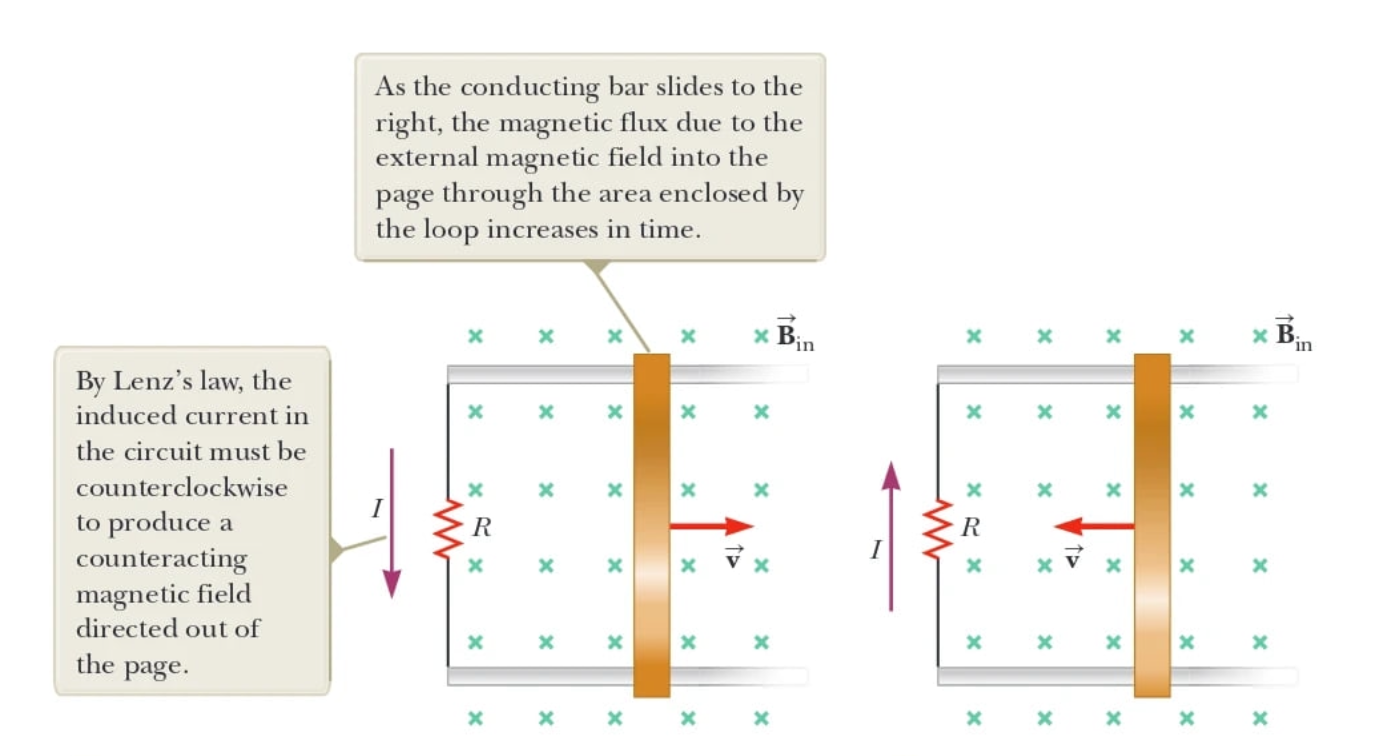
\includegraphics[scale=0.5]{lenz_law.png}
\end{center}
\subsection{Inductance}
\hrulefill

\paragraph*{Self-Inductance}
Self-inductance is the property of a circuit that causes it to generate an electromotive force in response to a change in current. It is measured in henries $[H] = [V\cdot \frac{s}{A}]$. The electromotive force generated by self-inductance is given by the following equation.

\begin{align*}
    \varepsilon_L &= -L\frac{dI}{dt}\\
    L &= \frac{\varepsilon_L}{dI/dt} = \frac{N\Phi_B}{I}
\end{align*}

Where $\varepsilon_L$ is the electromotive force generated by self inductance in volts, $L$ is the self-inductance in henries, $I$ is the current in amperes, $N$ is the number of turns in the coil, and $\Phi_B$ is the magnetic flux in webers.\\

\subsubsection*{RL Circuits}
\paragraph*{Definition}
An RL circuit is a circuit that contains a resistor and an inductor. When a current is passed through the circuit, the inductor generates
an electromotive force that opposes the change in current. This causes the current to increase more slowly than it would in a circuit with
only a resistor. The current in an RL circuit is given by the following equation.

\begin{align*}
    I(t) &= \frac{\varepsilon}{R}(1 - e^{-t/\tau})\\
    \tau &= \frac{L}{R}\\
    I_{max} &= \frac{\varepsilon}{R} 
\end{align*}

Where $I(t)$ is the current in amperes, $\varepsilon$ is the electromotive force in volts, $R$ is the resistance in ohms, $t$ is the time in seconds,
$\tau$ is the time constant in seconds, $L$ is the inductance in henries, and $I_{max}$ is the maximum current in amperes.\\


\paragraph*{Energy in a Magnetic Field}
The energy stored in a magnetic field is given by the following equation.

\begin{align*}
    U_B &= \frac{1}{2}LI^2
\end{align*}

Where $U_B$ is the energy stored in the magnetic field in joules, $L$ is the inductance in henries, and $I$ is the current in amperes.\\

\paragraph*{Energy in a Solinoid in a Magnetic Field}
\begin{align*}
    u_B = \frac{U_B}{V} = \frac{B^2V}{2\mu_0}
\end{align*}

Where $u_B$ is the energy density in the magnetic field in joules per cubic meter, $U_B$ is the energy stored in the magnetic field in joules, 
$V$ is the volume of the solenoid in cubic meters, $B$ is the magnetic field in teslas, and $\mu_0$ is the permeability of free space in henries per meter.\\


\paragraph*{Mutual Inductance}
Mutual inductance is the property of a circuit that causes it to generate an electromotive force in response to a change in current in a
neighboring circuit. It is measured in henries. 


\begin{align*}
    M_{12} &= \frac{N_2\Phi_12}{I_1} &M_{21} = \frac{N_1\Phi_21}{I_2}\\
    \varepsilon_1 &= -M_{21}\frac{dI_2}{dt} &\varepsilon_2 = -M_{12} \frac{dI_1}{dt}
\end{align*}

Where $M_{12}$ is the mutual inductance from circuit 1 to circuit 2 in henries, $N_2$ is the number of turns in circuit 2, $\Phi_{12}$ is the magnetic flux
from circuit 1 to circuit 2 in webers, $I_1$ is the current in circuit 1 in amperes, $M_{21}$ is the mutual inductance from circuit 2 to circuit 1 in henries
$N_1$ is the number of turns in circuit 1, $\Phi_{21}$ is the magnetic flux from circuit 2 to circuit 1 in webers, $I_2$ is the current in circuit 2 in
amperes, $\varepsilon_1$ is the electromotive force generated in circuit 1 in volts, $\varepsilon_2$ is the electromotive force generated in circuit 2 in
volts, and $M_{12}$ is the mutual inductance from circuit 1 to circuit 2 in henries.\\


\paragraph*{Oscillations in an LC Circuit}
An LC circuit is a circuit that contains a capacitor and an inductor. When a charge is passed through the circuit, the capacitor stores energy in the form of 
an electric field. When the capacitor is fully charged, the inductor generates an electromotive force that causes the charge to flow in the opposite direction.
This causes the capacitor to discharge, and the cycle repeats. Note that this cycle is between electric potential energy and magnetic poteneial
energy. The charge in an LC circuit is given by the following equation.

\begin{align*}
    q(t) &= Q_{max}\cos(\omega t + \phi)\\
    \omega &= \frac{1}{\sqrt{LC}}\\
    I &= \frac{dq}{dt} = -\omega Q_{max}\sin(\omega t + \phi) = -I_{max}\sin(\omega t + \phi)
\end{align*}

Where $q(t)$ is the charge in coulombs, $q_{max}$ is the maximum charge in coulombs, $\omega$ is the angular frequency in radians per second, $L$ is the 
inductance in henries, $C$ is the capacitance in farads, and $t$ is the time in seconds.\\

\subsubsection*{RLC Circuits}
An RLC circuit is a circuit that contains a resistor, an inductor, and a capacitor. When a charge is passed through the circuit, the capacitor stores energy 
in the form of an electric field. When the capacitor is fully charged, the inductor generates an electromotive force that causes the charge to flow in the 
opposite direction. This causes the capacitor to discharge, and the cycle repeats. The energy model for this circuit is given by the following equation.

\begin{align*}
    \Delta U_E + \Delta U_B + \Delta \varepsilon_{int} &= 0\\
    L\frac{d^2q}{dt^2} + R\frac{dq}{dt} + \frac{q}{C} &= 0
\end{align*}

Where $\Delta U_E$ is the change in electric potential energy, $\Delta U_B$ is the change in magnetic potential energy, and $\Delta \varepsilon_{int}$ is the change in internal energy.\\

The charge in an RLC circuit is given by the following equation.
\begin{align*}
    q(t) &= q_{max}e^{-\frac{R}{2L}t}\cos(\omega_d t + \phi)\\
    \omega_d &= \sqrt{\frac{1}{LC} - \frac{R^2}{4L^2}}
\end{align*}

Where $q(t)$ is the charge in coulombs, $q_{max}$ is the maximum charge in coulombs, $R$ is the resistance in ohms, $L$ is the inductance in henries, $C$ is the capacitance in farads, 
$\omega_d$ is the damped angular frequency in radians per second, and $t$ is the time in seconds.\\
\subsection{Electromagnetic Waves}
\hrulefill

\paragraph*{Definition}
Electromagnetic waves are waves of electric and magnetic fields that propagate through space. They are generated by accelerating charges 
and are characterized by their frequency and wavelength. Electromagnetic waves are governed by Maxwell's equations, which describe how electric
and magnetic fields interact with each other.

\paragraph*{Maxwell's Equations}

\begin{align*}
    \oint \vec{E} \cdot d\vec{A} &= \frac{Q_{enc}}{\varepsilon_0} &\text{Gauss's Law}\\
    \oint \vec{B} \cdot d\vec{A} &= 0 &\text{Gauss's Law in Magnetism}\\
    \oint \vec{E} \cdot d\vec{\ell} &= -\frac{d\Phi_B}{dt} &\text{Faraday's Law}\\
    \oint \vec{B} \cdot d\vec{\ell} &= \mu_0 I + \varepsilon_0\mu_0\frac{d\Phi_E}{dt} &\text{Ampere-Maxwell Law}
\end{align*}

Where $\vec{E}$ is the electric field in volts per meter, $\vec{B}$ is the magnetic field in teslas, $d\vec{A}$ is an infinitesimal 
segment of the circuit in meters, $Q_{enc}$ is the charge enclosed by the loop in coulombs, $\varepsilon_0$ is the permittivity of free 
space in farads per meter, $d\vec{\ell}$ represents an infinitesimal segment of the wire's length, $\Phi_B$ is the magnetic flux in webers, 
$\mu_0$ is the permeability of free space in henries per meter, $I$ is the current in amperes, and $\Phi_E$ is the electric flux in webers.\\

Note that if there is no current, $\mu_0 I = 0$, and the Ampere-Maxwell Law simplifies to:
\begin{align*}
    \oint \vec{B} \cdot d\vec{\ell} &= \varepsilon_0\mu_0\frac{d\Phi_E}{dt}
\end{align*}

\pagebreak

\subsubsection*{Electromagnetic Wave Equation}
The electromagnetic wave equation is a second-order partial differential equation that describes how electromagnetic waves propagate through space.
Assuming that the wave is propagating in the $x$ direction, the wave equation is given by the following system of equations.

\begin{align*}
    \large
\begin{cases}
    \frac{\partial^2\vec{E}}{\partial x^2} &= \mu_0\varepsilon_0\frac{\partial^2\vec{E}}{\partial t^2}\\
    \frac{\partial^2\vec{B}}{\partial x^2} &= \mu_0\varepsilon_0\frac{\partial^2\vec{B}}{\partial t^2}\\
    \frac{\partial^2 \vec{y}}{\partial x^2} &= \frac{1}{v^2}(\frac{\partial^2 \vec{y}}{\partial t^2})
\end{cases}
\end{align*}
    
Where $\vec{E}$ is the electric field in volts per meter, $\vec{B}$ is the magnetic field in teslas, $x$ is the position in meters, $t$ is the time 
in seconds, $\mu_0$ is the permeability of free space in henries per meter, $y$ is the wave function, $x$ is the position in meters and $\varepsilon_0$ 
is the permittivity of free space in farads per meter.\\

\paragraph{The Speed of Light}
The speed of light is the speed at which electromagnetic waves propagate through space. It is given by the following equation when the wave is propogating
through a vaccum.

\begin{align*}
    c_{vac} &= \frac{1}{\sqrt{\mu_0\varepsilon_0}} = 3.00 \times 10^8 \text{ m/s}
\end{align*}

\paragraph*{Solution to the Wave Equation}

\begin{align*}
    \frac{E_{max}}{B_{max}} &= c
\end{align*}

\paragraph{Poynting Vector}
The Poynting vector is a vector that describes the direction and magnitude of the energy flow in an electromagnetic wave. It is given by the following equation.

\begin{align*}
    \vec{S} &= \frac{1}{\mu_0}\vec{E} \times \vec{B}
\end{align*}

Where $\vec{S}$ is the Poynting vector in watts per square meter, $\vec{E}$ is the electric field in volts per meter, $\vec{B}$ is the magnetic field in teslas,
and $\mu_0$ is the permeability of free space in henries per meter.


\paragraph{Energy Carried by Electromagnetic Waves}
The energy carried by an electromagnetic wave is given by the following equation.

\begin{align*}
    U_E &= \frac{1}{2}\varepsilon_0E_{max}^2\\
    U_B &= \frac{1}{2\mu_0}B_{max}^2\\
    I &= S_{avg} = \frac{cB_{max}^2}{2\mu_0} = \frac{c}{U_{avg}}
\end{align*}

\paragraph{Momentum and Radiation Pressure}
Electromagnetic waves carry momentum and exert a pressure on objects they interact with. The momentum carried by an electromagnetic wave is given by the following 
equations.

\begin{align*}
    P &= \frac{S}{c} &\text{(Complete Absorption)}\\
    P &= \frac{2S}{c} &\text{(Complete Reflection)}\\
    P &= (1 + f) \frac{S}{c} &\text{(Partial Absorption)}
\end{align*}

Where $P$ is the momentum in newton-seconds, $S$ is the Poynting vector in watts per square meter, $c$ is the speed of light in meters per second, 
and $f$ is the fraction of the wave that is absorbed (check this one for accuracy).



\end{document}